\PassOptionsToPackage{dvipsnames}{xcolor}
\documentclass[aspectratio=169]{beamer}

\mode<presentation> {

\usetheme{Montpellier} % good one
\usecolortheme{beaver}

%\setbeamertemplate{footline} % To remove the footer line in all slides uncomment this line
\setbeamertemplate{footline}[page number] % To replace the footer line in all slides with a simple slide count uncomment this line

\setbeamertemplate{navigation symbols}{} % To remove the navigation symbols from the bottom of all slides uncomment this line
}

\setbeamertemplate{caption}[numbered]
\setbeamerfont{caption}{size=\scriptsize}
%\usepackage{etex}
\usepackage{array} 
\usepackage{graphicx} % Allows including images
\usepackage{booktabs} % Allows the use of \toprule, \midrule and \bottomrule in tables
\usefonttheme{professionalfonts}
\usepackage{mathptmx}
\usepackage{caption}
\usepackage{subcaption}
\usepackage{amsmath,amsthm,amssymb}
\usepackage{float}
% ------------------ My own stuff
\usepackage[utf8]{inputenc}
\usepackage[T1]{fontenc}

\usepackage{amsmath,amsthm,amssymb}
\DeclareMathOperator*{\argmax}{\arg\!\max}
\DeclareMathOperator*{\argmin}{\arg\!\min}
\DeclareMathOperator{\E}{\mathbb{E}}
\DeclareMathOperator{\R}{\mathbb{R}}

\beamertemplatenavigationsymbolsempty

\usepackage{rotating}
\usepackage{tikz}
\usepackage{fancyvrb}
\usepackage{listings}
\usepackage{verbatim}

\newcommand\blfootnote[1]{%
	\begingroup
	\renewcommand\thefootnote{}\footnote{#1}%
	\addtocounter{footnote}{-1}%
	\endgroup
}


%------------------
%	TITLE PAGE
%------------------

\title[CALTeC for CI]{CALTeC : Content-Adaptive Linear Tensor Completion
\\ for \\ Collaborative Intelligence}
\subtitle{\small ICIP 2021. Paper ID: 3013} % The short title appears at the bottom of every slide, the full title is only on the title page

\author[Hans]{Ashiv Dhondea, Robert A. Cohen and Ivan V. {Bajić}}% Your name
\institute[SFU-Multimedia Lab] 
{
\small
Multimedia Lab\\School of Engineering Science\\Simon Fraser University \\ % Your institution for the title page
\smallskip
\centering

\includegraphics[scale=0.25]{SFUhorizontallogorgb.pdf}
}

\date{\today} % Date, can be changed to a custom date

\begin{document}

\begin{frame}
\titlepage % Print the title page as the first slide
\end{frame}

\begin{frame}
\frametitle{Overview} % Table of contents slide, comment this block out to remove it
\tableofcontents % Throughout your presentation, if you choose to use \section{} and \subsection{} commands, these will automatically be printed on this slide as an overview of your presentation
\end{frame}

\section{Collaborative Intelligence}
%\begin{frame}
	%\frametitle{Introduction: Collaborative Intelligence}
	%\begin{figure}[H]
		%\centering
		%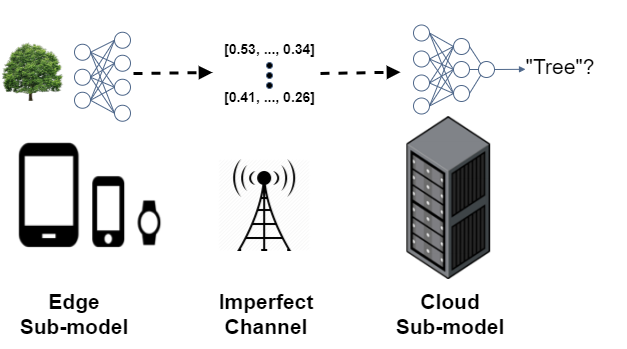
\includegraphics[scale=0.3]{image--000.png}
		%\caption{Blueprint for Collaborative Intelligence.\blfootnote{\tiny{Y. Kang, J. Hauswald, %C. Gao, A. Rovinski, T. Mudge, J. Mars, and L. Tang, “Neurosurgeon: Collaborative %intelligence between the cloud and mobile edge,” SIGARCH Comput. Archit. News, vol. 45, p. %615–629, Apr. 2017.}} \cite{neurosurgeon}}
	%	\label{fig:ci}
	%\end{figure}
	%CI has shown promising potential for latency and energy savings compared to purely cloud-based %or edge-based analysis solutions \cite{neurosurgeon,jointdnn}.
%\end{frame}

\begin{frame}
	\frametitle{Introduction: Collaborative Intelligence}
		\begin{figure}
		\begin{minipage}{.48\textwidth}
			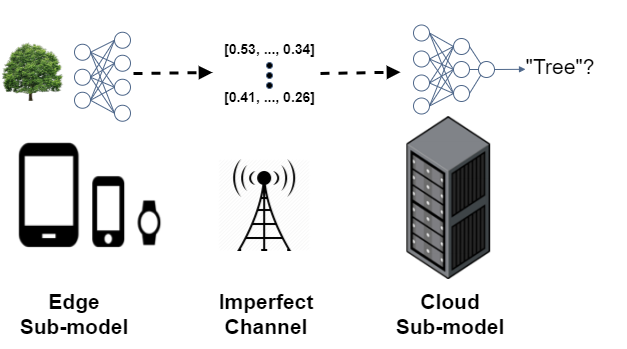
\includegraphics[width=\linewidth]{image--000.png}
			\caption{Blueprint for Collaborative Intelligence. \cite{neurosurgeon}}
		\end{minipage}\hfill
		\begin{minipage}{.48\textwidth}
		\begin{itemize}
		    \item Collaborative Intelligence (CI) leverages edge-based \& cloud-based resources to bring ``AI to the edge". 
		    \item CI has shown promising potential for latency and energy savings compared to purely cloud-based or edge-based analysis solutions \cite{neurosurgeon,jointdnn}.
		\end{itemize}
		\end{minipage}
		\blfootnote{\tiny \textsuperscript{1} Y. Kang, J. Hauswald, C. Gao, A. Rovinski, T. Mudge, J. Mars, and L. Tang, “Neurosurgeon: Collaborative intelligence between the cloud and mobile edge,” SIGARCH Comput. Archit. News, vol. 45, p. 615–629, Apr. 2017.}
		\blfootnote{\tiny \textsuperscript{2} A. E. Eshratifar, M. S. Abrishami, and M. Pedram, “JointDNN: An efficient training and inference engine for intelligent mobile cloud computing services,” IEEE Trans. Mobile Computing, vol. 20, no. 2, pp. 565–576, Feb. 2021.}
	\end{figure}
\end{frame}

\begin{frame}
    	\frametitle{System overview: collaborative intelligence.}
	\begin{figure}[H]
		\centering
		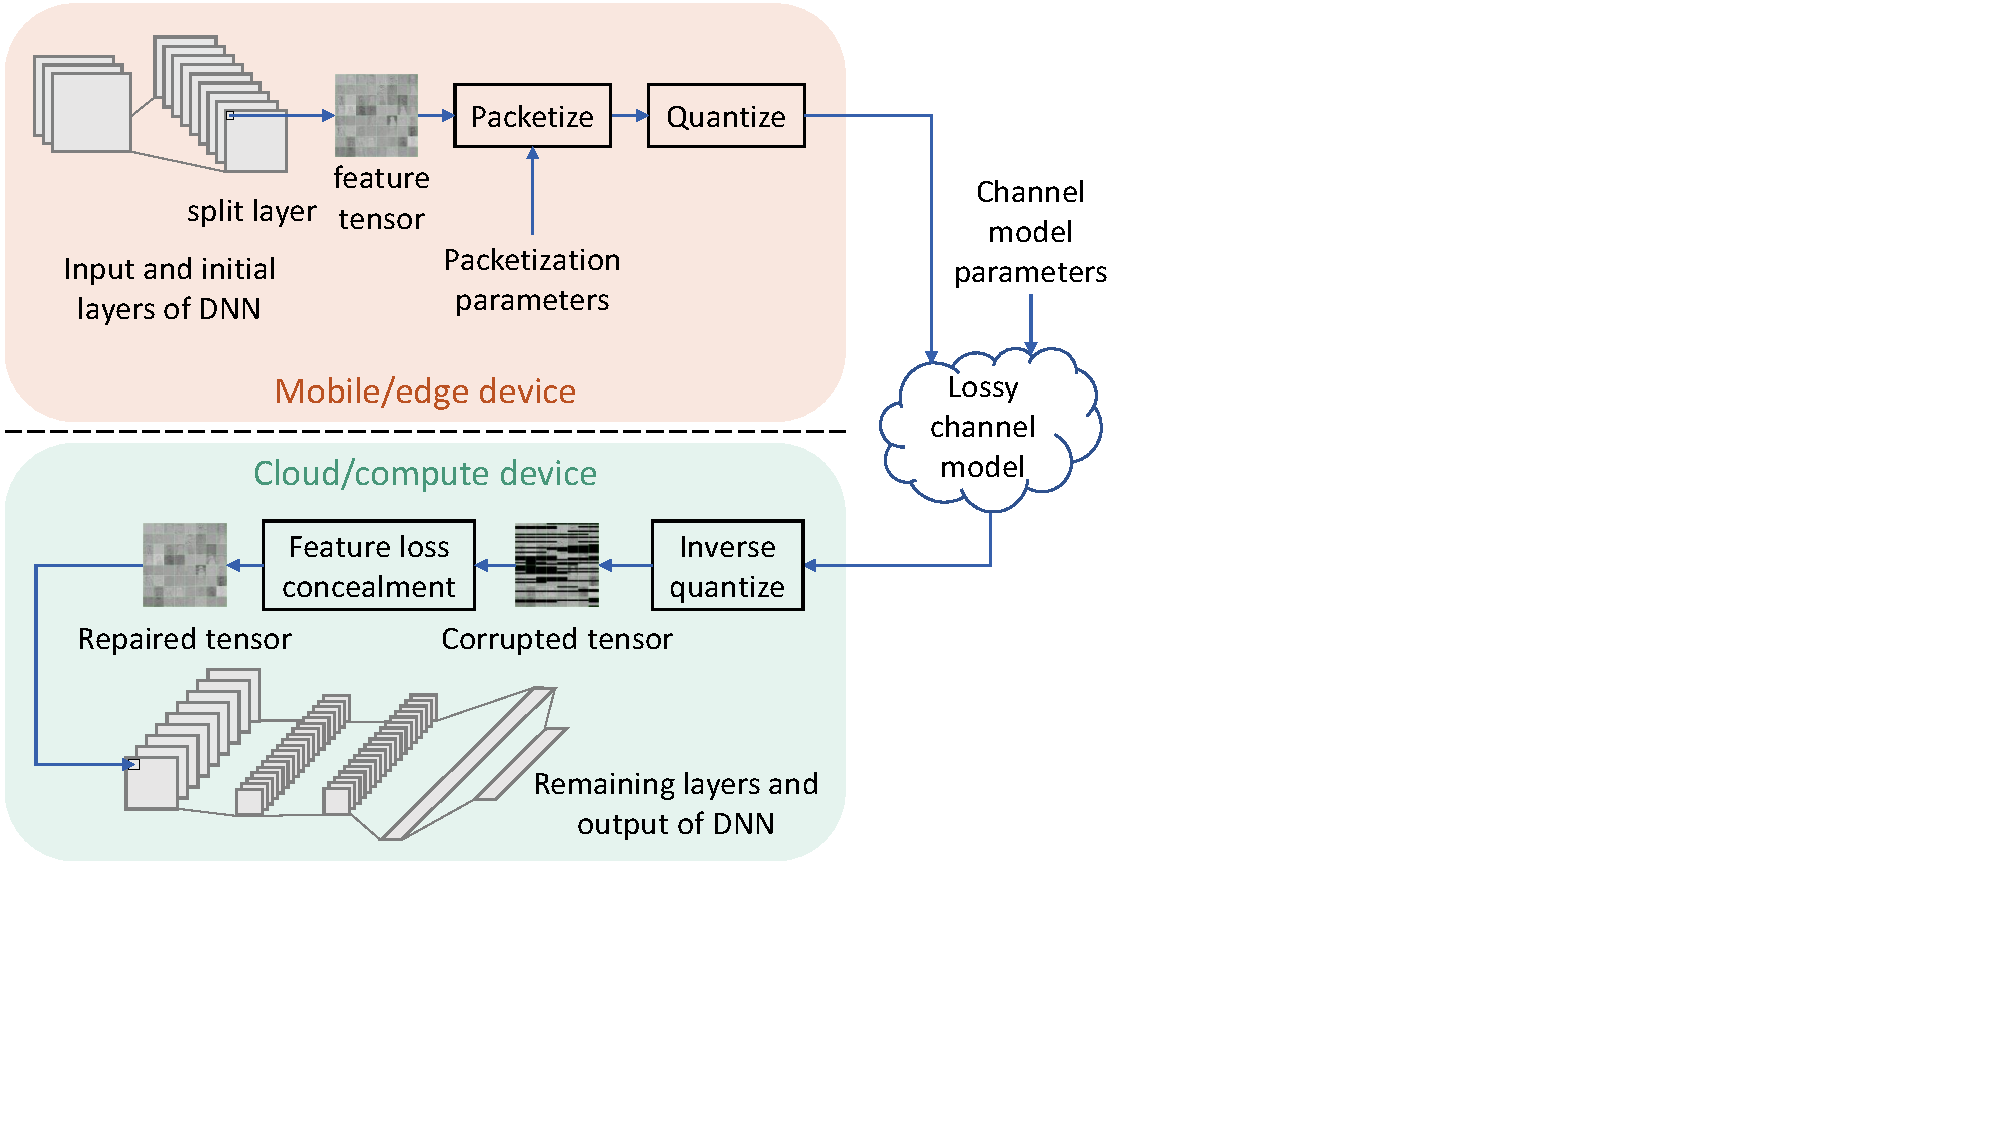
\includegraphics[scale=0.33,viewport=2.391047 126.719996 531.251984 538.217984,clip]{systemoverviewtv3.pdf}
		\caption{Deep feature tensor transmission overview (adapted from \cite[Fig. 1]{cohen2021lightweight})\blfootnote{\tiny \textsuperscript{3} R. A. Cohen, H. Choi, and I. V. Bajić, “Lightweight compression of intermediate neural network features for collaborative intelligence,” IEEE Open Journal of Circuits and Systems, vol. 2, pp. 350–362, 2021.}}
	\end{figure}
\end{frame}

\section{Literature review}

\begin{frame}
\frametitle{Intermediate tensor transmission over communication channels}
	\begin{itemize}
	\item Deep Feature Transmission Simulator (DFTS) was developed to simulate packet-based transmission of deep features over unreliable communication channels \blfootnote{\tiny \textsuperscript{4} H. Unnibhavi, H. Choi, S. R. Alvar, and I. V. Bajić, “Dfts: Deep feature transmission simulator,” 2018.} \cite{unnibhavi2018dfts}.
		\item DFTS has recently be updated for compatibility with TensorFlow version 2.
		\item Tensor completion can now be included in DFTS experiments.
	\end{itemize}
\end{frame}

\begin{frame}
	\frametitle{Packet loss concealment}
	\begin{itemize}
		\item General tensor completion methods, such as SiLRTC (Simple Low Rank Tensor Completion) and HaLRTC (High accuracy Low Rank Tensor Completion) \cite{liu2012tensor}\blfootnote{\tiny \textsuperscript{5} J. Liu, P. Musialski, P. Wonka, and J. Ye,``Tensor completion for estimating missing values in visual data,” IEEE transactions on pattern analysis and machine intelligence, vol. 35, no. 1, pp. 208–220, 2012.}.
		\item Method tailored for intermediate feature tensors: ALTeC - Adaptive Linear Tensor Completion \cite{Bragile2020} \blfootnote{\tiny \textsuperscript{6} L. Bragilevsky and I. V.Bajić,``Tensor completion methods for collaborative intelligence,” IEEE Access, vol. 8, pp. 41162–41174, 2020.}
		%\item Image inpainting methods such as Navier-Stokes based inpainting \cite{navierstokes} \blfootnote{\tiny \textsuperscript{6} M. Bertalmio, A. L. Bertozzi, and G. Sapiro, ``Navier-Stokes, fluid dynamics, and image and video inpainting,” in Proc. IEEE/CVF CVPR, vol. 1, pp. I–355–I–362, 2001.}
	\end{itemize}
\end{frame}

\begin{frame}
	\frametitle{Gilbert-Elliott (GE) communication channel model}
		\begin{figure}
		\begin{minipage}{.37\textwidth}
			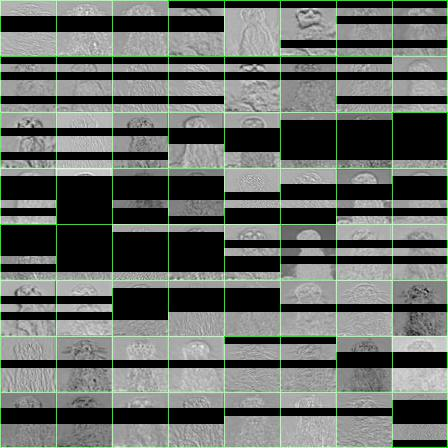
\includegraphics[width=0.77\linewidth]{tileddamagedgridm.jpg}
			\caption{Corrupted ResNet-18 deep feature tensor.}
		\end{minipage}\hfill
		\begin{minipage}{.6\textwidth}
		\small Two-state Markov model with a good (G) state and a bad (B) state. Parameters: burst loss probability ($P_B$) \& average burst length ($B_L$).
			\begin{align}
p_{B\to G} & = \frac{1}{L_B} & p_{B\to B} & =1-p_{B\to G} \label{eq:ge:1}
\end{align}
\begin{align}
p_{G\to B} & = \frac{P_B}{L_B(1-P_B)} & p_{G\to G} & = 1-p_{G\to B} \label{eq:ge:2}
\end{align}
\small 	The Gilbert-Elliott model has been shown to fittingly \mbox{capture} real-time observed packet loss patterns over the \mbox{Internet}. \cite{5755057}
		\end{minipage}
		\blfootnote{\tiny \textsuperscript{7} G. Hasslinger and O. Hohlfeld, “The gilbert-elliott model for packet loss in real time services on the internet,” in 14th GI/ITG Conference - Measurement, Modelling and Evaluation of Computer and Communication Systems, pp. 1–15, 2008.} 
	\end{figure}
\end{frame}

\section{Preliminaries}
\begin{frame}
	\frametitle{A deep feature tensor}
	\begin{figure}[H]
		\centering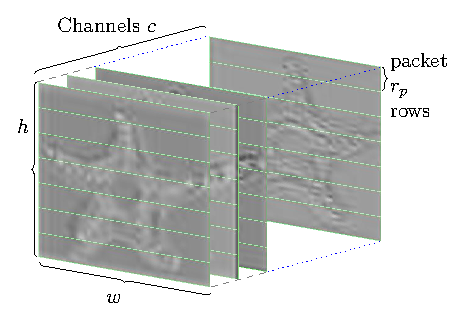
\includegraphics[scale=0.9]{tensorlostviz3icip.pdf}
		\caption{Tensor $\mathcal{X}$ from layer add\_1 of ResNet-18. Several consecutive rows in each channel form a feature data packet.}
	\end{figure}
\end{frame}

\begin{frame}
	\frametitle{Quantizing deep feature tensors}
	\begin{block}{Quantization to $n$-bits}
		For each feature tensor element $x \in \mathcal{X}$
		\[
		x_{\text{quant}} = \Bigg \lfloor \frac{(x - \mathcal{X}_{\text{min}})}{( \mathcal{X}_{\text{max}} -  \mathcal{X}_{\text{min}})} \cdot 2^{n-1} \Bigg \rceil
		\]
		Feature tensors can be cast from 32-bit floats to unsigned 8-bit integers.
	\end{block}
\end{frame}

\begin{frame}
	\frametitle{Corrupted tensor visualization}
	\begin{figure}
		\begin{minipage}{.4\textwidth}
			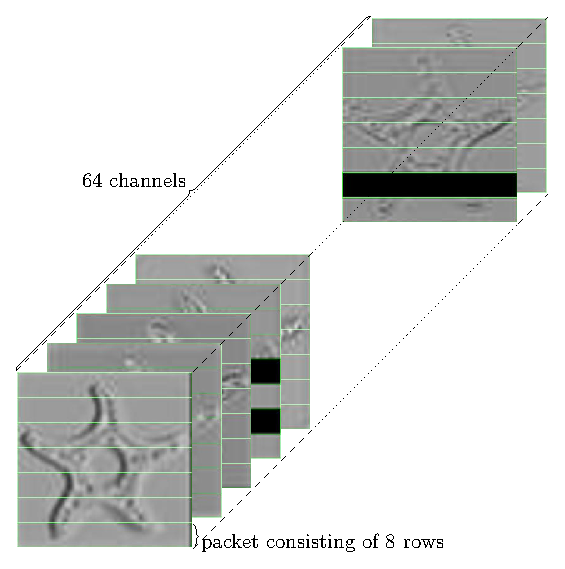
\includegraphics[width=0.75\linewidth]{tensorviz4.pdf}
			\caption{Corrupted ResNet-18 deep feature tensor consisting of 64 channels. Each channel consists of 7 packets. Packets are $8 \times 56$ blocks of deep feature tensor values.}
		\end{minipage}\hfill
		\begin{minipage}{.4\textwidth}
			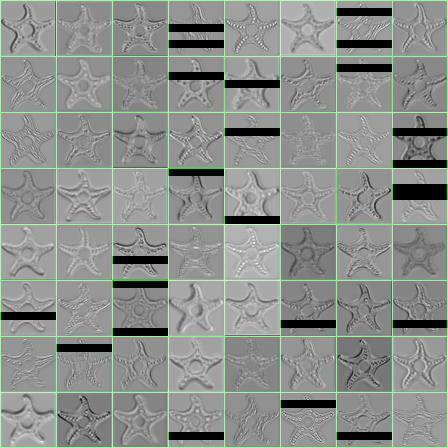
\includegraphics[width=0.78\linewidth]{tiledgridtensor.jpg}
			\caption{Tiled tensor $\tilde{\mathcal{X}} \in \mathbb{R}^{56 \times 56 \times 64}$ visualization. Each tile represents a channel of shape $56 \times 56$. }
		\end{minipage}
	\end{figure}
\end{frame}

\section{Proposed method}

\begin{frame}
	\frametitle{Principle behind CALTeC}
	\begin{figure}
		\begin{minipage}{.64\textwidth}
			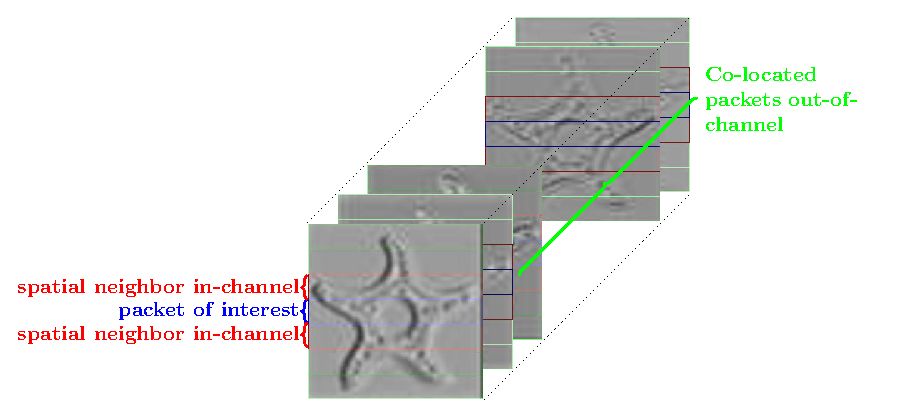
\includegraphics[width=\linewidth]{tensorvizcaltec.pdf}
			\caption{Tensor visualization for CALTeC rationale. The packet of interest (packet 3) is given by $\mathbf{x}_i^{(j)}$. The nearest spatial neighbor in-channel (either packet 2 or 4) is given by $\mathbf{x}_{i'}^{(j)}$.}
		\end{minipage}\hfill
		\begin{minipage}{.32\textwidth}
				\begin{block}{CALTeC assumption}
		The packet of interest can be obtained by selecting a locally similar co-located packet out-of-channel and applying an affine transformation to it. 
	\end{block}
		\end{minipage}
	\end{figure}
\end{frame}

\begin{frame}
	\frametitle{Selecting a candidate packet}
	\begin{block}{Locally similar candidate packet}
		We want to find another channel $k$ in the tensor that is locally similar to channel $j$. To measure local similarity, we use the Pearson correlation coefficient between the neighboring packet in-channel $\mathbf{x}_{i'}^{(j)}$ and its co-located packet out-of-channel $\mathbf{x}_{i'}^{(k)}$.
		\[
		 k^* = \underset{k}{\argmax} \frac{\left(\mathbf{x}_{i'}^{(j)}-\mu_{i'}^{(j)}\right)^\top \left(\mathbf{x}_{i'}^{(k)}-\mu_{i'}^{(k)}\right)}{\sigma_{i'}^{(j)}\sigma_{i'}^{(k)}},
		\label{eq:Pearson_coefficient}
		\]
		which means that the selected candidate packet is $\mathbf{x}_i^{(k^*)}$
	\end{block}
\end{frame}


\begin{frame}
	\frametitle{Transforming the candidate packet}
	\begin{block}{Finding the affine parameters}
		The selected candidate packet is adjusted to obtain the recovered packet.
		\[
		\widehat{\mathbf{x}}_i^{(j)} = a^*\cdot \mathbf{x}_i^{(k^*)} + b^*.
		\label{eq:recovered_packet}
		\]
		Affine parameters $\begin{bmatrix}a^*&b^* \end{bmatrix}$ are found by a least squares fit from $\mathbf{x}_{i'}^{(k^*)}$ to $\mathbf{x}_{i'}^{(j)}$.
	\end{block}
\end{frame}


\begin{frame}
	\frametitle{Example on recovering missing packet 3}
	\begin{figure}[H]
		\centering
		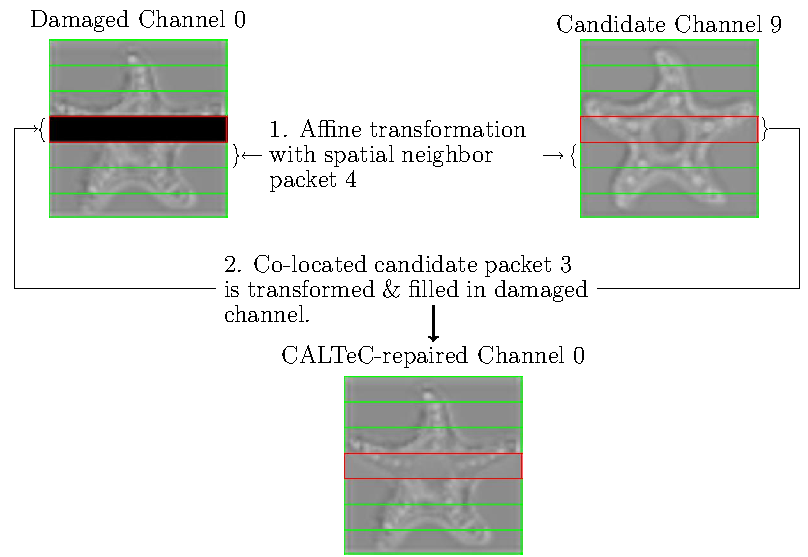
\includegraphics[scale=0.56]{lumimapcaltecnicer1.pdf}
		\caption{Illustration of CALTeC repairs on corrupted channel 0 of a deep feature tensor.}
	\end{figure}
\end{frame}

\begin{frame}
	\frametitle{CALTeC-repaired tensor}
	\begin{figure}[H]
		\centering
		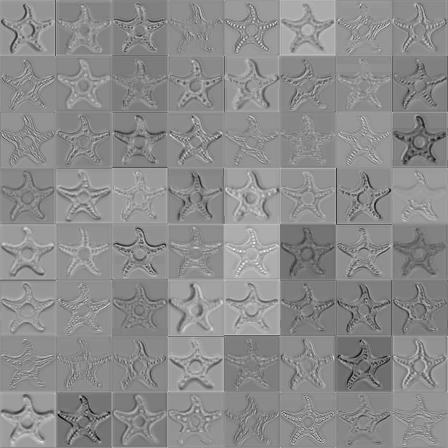
\includegraphics[scale=0.32]{caltecdemotiled.jpg}
		\caption{CALTeC repaired tensor}
	\end{figure}
\end{frame}


\section{Experiments}
\subsection{Visual results}

\begin{frame}
	\frametitle{Completed ResNet\nobreakdash-18 add\_1 tensors}
	\begin{figure}[H]
		\centering
		\begin{subfigure}{.17\linewidth}
			\centering
			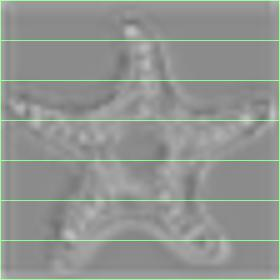
\includegraphics[width = 0.778\linewidth]{originalchannel1scaled.jpg}
			\caption{Original}
		\end{subfigure}%
		\hfill
		\begin{subfigure}{.17\textwidth}
			\centering
			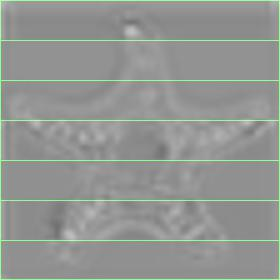
\includegraphics[width = 0.778\textwidth]{caltecrepairedchannel1scaled.jpg}
			\caption{CALTeC}
		\end{subfigure}%
        \hfill	
		\begin{subfigure}{.17\textwidth}
			\centering
			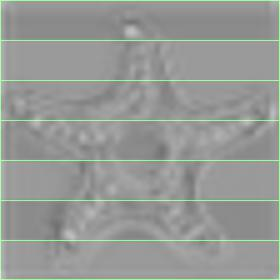
\includegraphics[width=0.778\textwidth]{altecrepairedchannel1scaled.jpg}
			\caption{ALTeC}
		\end{subfigure}
		
			\begin{subfigure}{.17\textwidth}
			\centering
			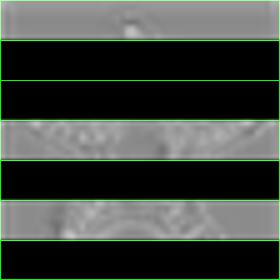
\includegraphics[width = 0.778\textwidth]{damagedchannel1scaled.jpg}
			\caption{Damaged channel.}
		\end{subfigure}%
		\hfill 
		\begin{subfigure}{.17\textwidth}
			\centering
			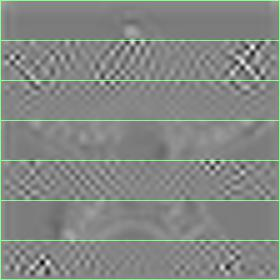
\includegraphics[width=0.778\textwidth]{silrtc50repairedchannel1scaled.jpg}
			\caption{SILRTC 50 iterations.}
		\end{subfigure}%
		\hfill
		\begin{subfigure}{.17\textwidth}
			\centering
			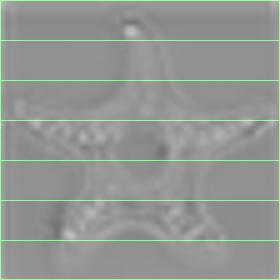
\includegraphics[width=0.778\textwidth]{halrtc50repairedchannel1scaled.jpg}
			\caption{HaLRTC 50 iterations.}
		\end{subfigure}
		\caption{Channel 1 in a damaged \textit{starfish} ResNet\nobreakdash-18 tensor. Images were mapped to grayscale and scaled up using bicubic interpolation for enhanced visualization)}
		\label{fig:expt:repair:demo}
	\end{figure}
\end{frame}

\subsection{Monte Carlo experiments}
\begin{frame}
\frametitle{Monte Carlo experiments}
\begin{figure}[H]
    \centering
    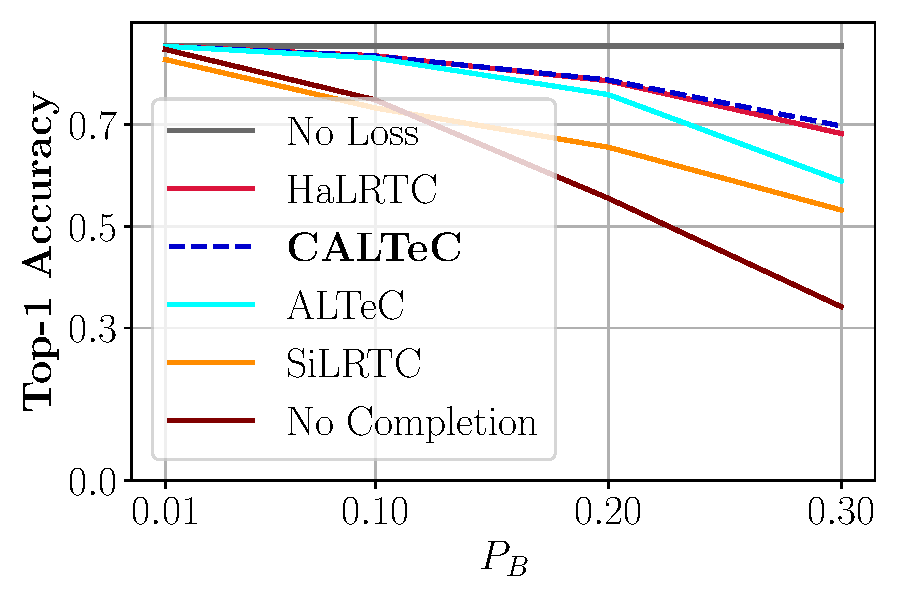
\includegraphics[scale=0.49]{add1fontsize20v2modified.pdf}
    \caption{ResNet\nobreakdash-18 add\_1 tensor completion results. Our proposed method, CALTeC, offers the best performance.}
    \label{fig:mcresnet18add1}
\end{figure}
\end{frame}

\begin{frame}
    \frametitle{Comparison of tensor completion methods}
    \begin{table}[b]
\caption{Tensor completion methods used in our experiments on ResNet\nobreakdash-18 tensors.}
\vspace{4pt}
    \label{tab:methods}
    \centering
    \begin{tabular}{l|c|c|r|r}
         Method & Iterative? & Pre-training? & \texttt{add\_1} & \texttt{add\_3} \\
         \hline
         SiLRTC~\cite{liu2012tensor}(per iter.)& Yes & No & $228.1~\mathrm{ms}$ & $122.1~\mathrm{ms}$ \\
         HaLRTC~\cite{liu2012tensor}(per iter.) & Yes & No & $242.6~\mathrm{ms}$ & $128.2~\mathrm{ms}$ \\
         ALTeC~\cite{Bragile2020} & No & Yes & $30.5~\mathrm{ms}$ & $102.0~\mathrm{ms}$ \\
         CALTeC & No & No & $77.5~\mathrm{ms}$ & $186.8~\mathrm{ms}$
    \end{tabular}
\end{table}
\end{frame}

\section{Conclusions}
\begin{frame}
	\frametitle{Conclusions and recommendations}
	\begin{itemize}
		\item CALTeC exploits intra- and inter-channel similarity in deep feature tensors to find the best candidates in other channels to fill in the gaps in corrupted packetized deep feature tensors.
		\item CALTeC adjusts the recovered data with an affine transformation.
		\item CALTeC is slower than ALTeC but unlike ALTeC, it does not require pre-training.
		\item Both ALTeC and CALTeC are much faster than SiLRTC and HaLRTC.
		\item Future work can focus on extending DFTS to run different tasks and to incorporate different compression methods for the transmitted deep feature tensor.
	\end{itemize}
\end{frame}

%------------------------------------------------
\section{Implementation}
\begin{frame}
\frametitle{Implementation \& Results}
Public repository for DFTS2: \url{https://github.com/AshivDhondea/DFTS_TF2}.

\begin{figure}[H]
    \centering
    
\includegraphics[scale=0.35]{frame.pdf}
\end{figure}

This repository also contains the packet loss traces and Monte Carlo experiment results presented in this paper.
	\end{frame}
	
%---------------------------------------------
\section{References}
\bibliographystyle{ieeetr}
\bibliography{icipcaltecrefs}
%-----------------------------------------------
\end{document} 